% Social Media Analytics 2022/23

%%%%%%%%%%%%%%%%%%%%%%%%%%%%%%%%%%%%%%%%%%%%%%%%%%%%%%

% OPTIONAL PACKAGES
\documentclass[12pt,journal,compsoc]{IEEEtran}
\usepackage{amsfonts}
\usepackage{caption}
\usepackage{multirow}
\usepackage[table,xcdraw]{xcolor}
\usepackage{booktabs}
\usepackage{tabularx}
\usepackage[hyphens]{url}
\usepackage{biblatex}
\usepackage{blindtext,graphicx}
\usepackage[absolute]{textpos}
\usepackage[italian]{babel}
\usepackage{float}

\addbibresource{ref.bib} %Import the bibliography file

%%%%%%%%%%%%%%%%%%%%%%%%%%%%%%%%%%%%%%%%%%%%%%%%%%%%%%

\begin{document}

\begin{textblock}{5}(1,0.5)
\noindent\small Social Media Analytics - UniMib 2022/23
\end{textblock}

\title{Smart Working\\
\vspace{2mm}\large{Social Network and Content Analysis}}
\author{Agazzi Ruben 844736\\Cominetti Fabrizio 882737}

\IEEEtitleabstractindextext{%
\begin{abstract}
Negli ultimi anni il tema legato allo \textit{smart working} ha assunto una caratura di primo rilievo nelle discussioni in ambito lavorativo. Dalla necessità nel periodo di pandemia alle richieste di lavoratori che, una volta ristabilità la situazione sanitaria post-pandemia, non hanno voluto rinunciare a tale possibilità, considerata un vantaggio nel proprio equilibrio tra vita privata e lavoro. Ma il tema è discusso anche per i vantaggi offerti alle aziende, soprattutto in termini di risparmio su strutture ed energie, oppure ancora per questioni legate a traffico e inquinamento. Insomma, lo smart working non può più essere considerato un tema di secondo piano. Per questo motivo, abbiamo voluto analizzare il sentiment e le community degli utenti relativamente al tema, specialmente dopo gli ultimi interventi a livello governativo che hanno parzialmente ridotto la possibilità di usufruire dello smart working.
\end{abstract}}

\maketitle
\IEEEpeerreviewmaketitle
\IEEEdisplaynontitleabstractindextext

\tableofcontents

%%%%%%%%%%%%%%%%%%%%%%%%%%%%%%%%%%%%%%%%%%%%%%%%%%%%%%

\section{Introduction}
\IEEEPARstart{L}{o} Smart Working, anche conosciuto come lavoro agile, indica \textit{una modalità di esecuzione del rapporto di lavoro subordinato caratterizzato dall'assenza di vincoli orari o spaziali e un'organizzazione per fasi, cicli e obiettivi, stabilita mediante accordo tra dipendente e datore di lavoro; una modalità che aiuta il lavoratore a conciliare i tempi di vita e lavoro e, al contempo, favorire la crescita della sua produttività} \cite{Gazzetta} \cite{MIUR}.\\
Lo smart working è un modello organizzativo in grado di portare notevoli vantaggi alle organizzazioni che lo adottano: in termini di produttività, di raggiungimento degli obiettivi, ma anche in termini di welfare e qualità della vita del lavoratore.\\
Già nel 2015, il British Standards Institution affermava che: \textit{"I principi dello smart working riconoscono che la tecnologia e i modelli di lavoro flessibile stanno cambiando in meglio il modo in cui lavoriamo} \cite{BSI}.\\
Guardando all'altra faccia della medaglia, ricerche come quella condotta da NordVPN nel 2020, hanno portato alla luce alcuni rischi per i lavoratori, tra cui un involontario aumento di ore lavorative, l'isolamento dell'individuo e la difficoltà dello stesso di separare vita sociale e attività lavorativa, oltre a pericoli legati al tema privacy e sicurezza \cite{Forbes}.\\
Tra fine 2021 e inizio 2022, si stimavano intorno ai 2,9 milioni i cosiddetti "smart worker" in Italia, in aumento rispetto ai 1,15 milioni di fine 2019 ma in calo al giorno d'oggi e su un totale stimato di 8 milioni di potenziali usufruitori. La stessa ricerca mostra inoltre come l'Italia sia fanalino di coda nell'adozione dello smart working in Europa e abbia una media di gran lunga inferiore rispetto alla media UE considerando numero di individui e totale di giorni a settimana di lavoro agile \cite{Rai}.\\
A partire da febbraio 2020, a seguito del diffondersi dell'epidemia Covid-19 del Coronavirus, sono stati emanati dal Governo una serie di provvedimenti per semplificare l'accesso allo Smart Working e diffonderne al massimo l'utilizzo. La pandemia ha infatti costretto numerosi lavoratori a fronteggiare l'emergenza sanitaria tramite lo smart working.\\
I numeri enunciati sopra fanno pensare che, una volta finita la fase più dura dell'emergenza - con misure tra le quali il lockdown - la maggior parte di aziende e lavoratori abbiano scelto di tornare alle modalità di lavoro tradizionali.\\
L'opinione pubblica è divisa tra chi ha preferito continuare ad usufruire di una modalità di lavoro agile anche in seguito, sottolineandone i numerosi benefici, e chi, con un parere opposto, sostiene l'importanza della comunicazione face-to-face e considera insostituibile l'interazione umana giornaliera, oppure ancora vorrebbe cedere il passo a nuovi strumenti e tecnologie.\\
In aggiunta a tutto ciò, è anche opportuno precisare che solo alcune tipologie di lavoratori possono svolgere con continuità una modalità di lavoro agile, principalmente i lavoratori d'ufficio, mentre altri hanno dunque un interesse marginale per l'argomento.\\
Oltre alla già citata pandemia, le direttive annesse per i lavoratori e le varie proroghe allo stato d'emergenza e allo smart working in regime semplificato, hanno portato alla ribalta, una volta di più, il fenomeno.\\
Il Governo ha infatti prorogato negli ultimi giorni del 2022 il diritto allo smart working con un emendamento dedicato in Manovra soltanto per i lavoratori considerati "fragili" del pubblico e del privato. Dunque, dicendo addio ai giorni di lavoro da casa per i genitori di figli under 14, fino a prima di questo emendamento compresi nella misura varata dal precedente Esecutivo, e che dall’1 gennaio sono dovuti tornare a contrattare individualmente i giorni di lavoro da remoto con la propria azienda.\\
La decisione del Governo di escludere dalla misura i genitori di figli under 14 è spiegata dal venire meno delle misure anti-Covid adottate durante la pandemia, sulle quali si basava la necessità di ricorrere al lavoro da remoto per milioni di lavoratori.\\
La nostra analisi vuole dunque concentrarsi su questo periodo finale, tra la fine del 2022 e l'inizio del 2023, per indagare le reazioni, il sentiment e le emozioni riversate sulla rete - Twitter nel nostro caso - in seguito all'annuncio di queste decisioni.\\
Per concludere, il progetto vuole rispondere a domande quali \textit{Come è rappresentato il panorama italiano intorno al tema su Twitter? Quali sono gli utenti più influenti al suo interno? Qual è stato il sentiment generale nel periodo preso in considerazione? Quali sono state le emozioni e le diverse reazioni nei giorni intorno all'annuncio del Governo sull'ulteriore riduzione dello Smart Working?}

\section{Data Collection}
Per costruire il dataset, necessario per rispondere alle domande di progetto, abbiamo scaricato un totale di 2667 tweet dal social network Twitter, tramite l'utilizzo dell'API fornita dallo stesso social.\\
I dati sono stati scaricati utilizzando un jupyter notebook e la libreria Tweepy, che permette di effettuare il download di tweet corrispondenti ad uno o più hashtag o keyword. Nel nostro caso, abbiamo scelto di utilizzare le seguenti keyword: \textit{"smartworking" OR "remotework" OR "lavoroagile" OR "hybridwork" OR "smart working" OR "remote work" OR "lavoro agile"}.\\
Siccome il tema è dibattuto e rigurda in particolare modo l'Italia, abbiamo scelto di svolgere lo studio su tweet in lingua italiana, scaricando dunque solamente i tweet nella lingua selezionata.\\
L'API permette di scaricare tweet con alcune limitazioni relative al numero di giorni e alle richieste di download consecutive. Il periodo d'interesse va dal 26 dicembre 2022 al giorno 5 gennaio 2023. Il periodo considera dunque anche giorni iniziali in cui alcune voci in merito iniziavano ad emergere e un periodo successivo dopo l'annuncio ufficiale. Come possiamo osservare dalla seguente distribuzione, il giorno con il maggior numero di tweet pubblicati è il giorno 30/12/2022, penultimo giorno di lavoro agile concesso anche ai genitori di figli U14 e giorno in cui l'opzione - obbligatoria - di tornare in ufficio si avvicinava sempre più per moltissimi italiani.

\begin{figure}[H]
  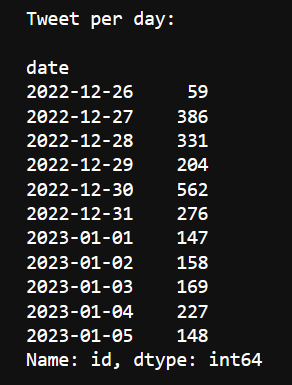
\includegraphics[scale=1]{./images/tweetxday.png}
  \caption{Number of Tweets per Day}
\end{figure}

Il dataset iniziale, esportato e salvato in csv, si compone dunque di un totale di 10 variabili: $'date', 'id', 'text', 'like', 'n_rt', 'author', 'location', 'retweeted', 'user_mentions', 'hastags'$.

\begin{itemize}
	\item \textit{date} : data e ora di pubblicazione del tweet
	\item \textit{id} : identificatore unico del tweet
	\item \textit{text} : testo contenuto nel tweet, estratto tramite l'opzione extended
	\item \textit{like} : numero di like
	\item \textit{n\_rt} : numero di retweet
	\item \textit{author} : nome utente dell'autore del tweet
	\item \textit{location} : localizzazione di pubblicazione del tweet, non sempre disponibile
	\item \textit{retweeted} : valore booleano, 'true' se si tratta di un retweet, 'false' altrimenti
	\item \textit{user\_mentions} : menzioni di altri utenti contenute nel tweet
	\item \textit{hastags} : hashtags utilizzati nel tweet
\end{itemize}

\subsection{Data Pre-Processing}
La prima operazione effettuata è stata di verificare l'eventuale presenza di duplicati, e l'eventuale rimozione degli stessi. Non sono presenti tweet duplicati, dunque il totale di tweet resta di 2667 elementi.\\
Il formato della variabile 'date' è stato processato e sono state estratte le variabili 'day', 'month', e 'year' per visualizzare il numero di tweet effettuati per giorno, come visto nell'immagine di cui sopra.\\
Dopodiché, abbiamo creato un dataframe all'interno di cui è stato svolto un conteggio di numero di tweet effettuati dallo stesso autore. Il risultato è visibile nell'immagine sottostante:

\begin{figure}[H]
  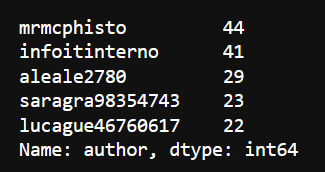
\includegraphics[scale=1]{./images/freq-authors.png}
  \caption{Number of Tweets per Author - Ordered}
\end{figure}

Da ogni tweet, abbiamo poi estratto la lista degli hashtags e delle menzioni contenute, inserite rispettivamente in due colonne del dataframe principale: $'hashtags_list', 'mentions'$.

Per ogni documento presente nel corpus, sono state svolte le operazioni di pre-processing necessarie per analizzare il testo. In particolare:

\begin{itemize}
	\item \textit{Remove Numbers} : rimozione dei numeri all'interno del testo
	\item \textit{Lower Text} : testo convertito in carattere minuscolo ('lower case')
	\item \textit{Lemmatization} : x
	\item \textit{Remove Punctuation} : x
	\item \textit{StopWords Deletion} : rimozione delle stopwords italiane
	\item \textit{Tokenization} : x
\end{itemize}

\section{Analysis}
\subsection{Social Network Analysis}
For the social network analysis we took the dataset of tweets we obtained from the twitter web api, and we kept only the columns relative to the tweet's author username and the list of users mentioned in the tweet. 
\subsubsection{Graph building}
We built our graph using the python library "NetworkX". Specifically we took every tweet in our dataset and for every tweet we took the tweet's author and users mentioned in the tweet, which becomes nodes of the graph, and then we make an edge between them. After this step we created inside our graph a total of 1820 nodes and 2568 edges between nodes.

\subsubsection{Nodes degree}
After building the graph we calculated the degree of every node inside the graph. The degree of a node of a graph is the number of edges that are incident to the node. After calculating the degree for every node we found out that the maximum degree found inside the graph is equal to 210 and the minimum degree found is equal to 1. 
\begin{table}[ht]
\centering
\begin{tabular}{c c }
	Node name & Degree  \\
	\hline
	BonomiAllegra & 210  \\
	mrmcphisto & 145  \\
	GiorgiaMeloni & 141  \\
	AlbertoBagnai & 118  \\
	ClaudioDurigon & 82  \\
\end{tabular}
\caption{First five nodes ordered by degree}
\end{table}

We also decided to calculate the average degree of the graph, which is equal to 2.82. Because the average degree is greater than we already assumed that there will be a giant component inside the graph. A giant component in graph theory is a connected component of a graph that contains a finite fraction of the entire graph's vertices.

\subsubsection{Assortativity}
Assortativity is a measure of how nodes inside a network connect to each other. If an interaction network is assortative nodes of comparable degree tent to link each other: bigger nodes(hubs) will tend to connect to hubs and smaller nodes will tend to connect to each other. If an interaction network is disassortative hubs wille tend to connect to small degree nodes, and small degree nodes will tend to connect to hubs. If the interaction network is neutral nodes will link to each other randomly.
We can calculate an assortativity coefficient of a graph; if this coefficient is greater than 0 the network is assortative, if is equal to 0 is neutral and if is less than 0 it is disassortative.
In out case the assortativity coefficient is equal to -0.244, which makes our network disassortative.

\subsubsection{Community detection}

\subsection{Social Content Analysis}
Per quanto riguarda la \textit{Social Content Analysis}, è stato utilizzato FEEL-IT, un dataset e un pacchetto per effettuare la \textit{Sentiment Analysis} e l'\textit{Emotion Recognition} in lingua italiana.\\
FEEL-IT è disponibile tramite un pacchetto Python \cite{FEEL-IT} e utilizza BERT, ...

%Fine-Tuning (Um)BERT(o). As standard in these recent pre-training times, we fine-tuned a BERT model with our proposed data set. BERT is one of the most popular neural architectures in Natural Language Processing. Fine-tuning BERT allows us to have a robust classification model to predict our labels. Fine-tuning is the operation that allows us to adjust the weights of the BERT model to perform our classification task.
%There are many different BERT models for many languages (see Nozza et al., 2020, for a review and BERTLang). Here, we use UmBERTo, a very efficient Italian BERT model. In particular, we fine-tuned the UmBERTo model trained on the Common Crawl data set.

%Recognizing emotions in text is fundamental to get a better sense of how people are talking about something. People can talk about a new event, but positive/negative labels might not be enough. There is a big difference between being angered by something and scared by something. This difference is why it is vital to consider sentiment and emotion in text.

Per quanto rigurda la \textit{Sentiment Analysis}, il pacchetto divide i tweet in 'positive' e 'negative', valori che sono stati assegnati ad una nuova colonna, chiamata 'sentiment\_BERT'. Inoltre, a seconda del valore assegnato dal modello, sono state create altre tre variabili, 'positive', 'negative', con valore 1 in caso di valore corrispondente al sentiment (quindi 1 alla colonna 'positive' in caso di sentiment individuato positivo) e 0 altrimenti, e 'ratio', di valore 1 in caso di sentiment positivo e -1 in caso di sentiment negativo. Il dataset così composto è stato salvato in un file csv per ulteriori analisi.\\
Il modello di \textit{Emotion Recognition} è in grado di individuare invece quattro emozioni: 'joy', 'fear', 'anger', 'sadness'. Il procedimento svolto è il medesimo per la sentiment analysis, e sono state dunque create quattro variabili, una per ogni emozione, con valore 1 in caso di tweet corrispondente alla stessa emozione, 0 altrimenti. Anche in questo caso, il dataset è stato esportato in file csv per ulteriori analisi.

\section{Visualization}
...

\section{Summary}
...

% risposta domande di ricerca

% per migliorare progetto: più giorni, classificazione neutra sentiment

%%%%%%%%%%%%%%%%%%%%%%%%%%%%%%%%%%%%%%%%%%%%%%%%%%%%%%%%%%%%%%%%%

\nocite{*}
\printbibliography

\end{document}